\documentclass[10pt]{article}

% ---------------------------------------------------------------
% REX preprint — arXiv position paper (cs.LG, cross-list cs.AI)
% Source of truth: docs/article_source_explicabilite.md
% Writing rules (section 13 of the source document):
%   - the vision and approach are the author's; format them, do not alter them
%   - ambitious on the framework, sober on the evidence
%   - every empirical claim points to a results table
%   - no claims about humans; real-data claims limited to the tables
%   - graph editing as learning = stated as an explicit conjecture
% ---------------------------------------------------------------

\usepackage[margin=1in]{geometry}
\usepackage[T1]{fontenc}
\usepackage[utf8]{inputenc}
\usepackage{mathptmx}
\usepackage{microtype}
\usepackage{graphicx}
\usepackage{booktabs}
\usepackage{amsmath,amssymb}
\usepackage{caption}
\usepackage{xcolor}
\usepackage{enumitem}
\setlist{itemsep=1pt,topsep=3pt,parsep=0pt}
\setlength{\textfloatsep}{12pt plus 2pt minus 2pt}
\setlength{\intextsep}{10pt plus 2pt minus 2pt}
\usepackage[numbers,sort&compress]{natbib}
\usepackage{xurl}
\usepackage[colorlinks=true,linkcolor=blue!60!black,citecolor=blue!60!black,urlcolor=blue!60!black]{hyperref}

\captionsetup{font=small,labelfont=bf}
\graphicspath{{figures/}}

\title{\bfseries Explainability is Relational:\\A Receiver-Dependent Framework for AI Interpretability}

\author{%
  Reda Azizi\\
  \small\texttt{redatln19@gmail.com}\\
  \small\url{https://github.com/RedaAZIZI/impact_social}%
}

\date{}

\begin{document}
\maketitle

% NOTE (not for publication): the extended abstract below implements the
% proposal of section 16 of the source document. It MUST be validated by
% the author before submission.
\begin{abstract}
Explainability in AI is treated as an intrinsic property of the model. We argue that this is a category error: explainability is a property of the \emph{relation} between a model $M$ and a receiver $R$, each endowed with its own representational basis. Classical XAI (feature attributions, surrogate trees) is the degenerate case in which the bases of $M$ and $R$ are assumed identical. We propose (i) a formal definition: $M$ is explainable for $R$ if and only if there exists a decision graph, expressed in $R$'s predicate vocabulary and of bounded complexity, that simulates $M$ to fidelity $\varepsilon$; (ii) a contrastive, composable \emph{why-operator} $W$ that turns explanation into an interactive protocol whose cost (number of questions) measures explainability; (iii) controlled experiments on a synthetic world whose explanatory ground truth is known. Results: the cost of explainability grows monotonically with the misalignment angle between bases (fidelity AUC $0.918 \to 0.745$); reconstructing $M$'s graph through successive why-questions converges in ${\sim}6$ questions under an aligned basis (fidelity $97.9\%$) and fails to converge under a misaligned one (plateau at $71\%$) --- same model, same answers: only the receiver's basis changes. On real data, the framework predicts where natural misalignment appears: absent on a credit-scoring task whose expert concepts do not carry the signal (a clean, pre-registered negative result), significant on a predictive-maintenance benchmark whose failure laws are written in compound physical quantities ($+0.046$, $p < 10^{-3}$) --- and modulated by the internal basis of the model itself. Finally, under continuous drift, a graph maintained through dialogue (one sentence per drift, zero labels) outperforms a network retrained on $75{,}000$ examples, with no cumulative forgetting: we conjecture learning by graph editing as a candidate post-gradient paradigm.
\end{abstract}

\section{Introduction: the hidden assumption of XAI}
\label{sec:intro}

Between humans, explanation works because a common ground --- language, concepts, culture --- is shared by default. That channel was never formalized because it never failed. With AI systems the assumption collapses: the internal features of a neural network do not coincide with human concepts. Yet the standard explainability toolbox --- SHAP~\citep{lundberg2017unified}, LIME~\citep{ribeiro2016why}, saliency maps, surrogate trees~\citep{craven1996extracting,frosst2017distilling} --- implicitly assumes that the axes of the model \emph{are} the concepts of the receiver. These methods compute an explanation in the basis of $M$ and deliver it, unchanged, to $R$.

\paragraph{Thesis.} \emph{Explainability is not a property of $M$. It is a property of the triple $(M, R, Q)$}: the model, the receiver's representational basis, and the contextual question being asked. Classical XAI is the special case $\mathrm{base}(M) = \mathrm{base}(R)$ with $Q =$ ``why this output?'' and no explicit contrast.

This paper is a position paper with preliminary evidence. Our contribution is threefold. First, a formal framework in which explainability is defined relative to a receiver and a question (Section~\ref{sec:framework}). Second, controlled experiments on a synthetic world whose explanatory ground truth is known by construction, showing that the cost of explanation is governed by the alignment between the bases of $M$ and $R$ --- not by $M$ alone (Section~\ref{sec:synthetic}). Third, two consequences of taking the relation seriously: on real data, the framework predicts \emph{where} natural misalignment appears, and we confirm both the positive and the negative prediction (Section~\ref{sec:real}); and because explanation is a channel, the same channel can be used in reverse --- we show that editing an explainable graph through dialogue outperforms gradient-based adaptation under drift, and we state the corresponding conjecture explicitly (Section~\ref{sec:interactive}).

If explanation is an interactive protocol --- a series of ``why?'' questions --- then the same channel serves learning: the inverse of the why-operator inserts graph fragments supplied by $R$ into $M$'s explainable graph. The long-term perspectives are (a) AI that learns in dialogue by graph editing --- local, instantaneous, traceable --- rather than by gradient descent; (b) contextual compression: a large model distilled on the fly, per context, into a small, locally executable, fully explainable graph; (c) personal AI that grows with its user. The performance--interpretability trade-off~\citep{rudin2019stop} is real but is usually evaluated on static benchmarks; in an interactive regime, a graph correctable in one sentence can beat a frozen network that requires retraining. This is a falsifiable thesis, and Sections~\ref{sec:synthetic}--\ref{sec:interactive} are its first controlled test.

\section{Formal framework}
\label{sec:framework}

\subsection{Definitions}
\label{sec:defs}

\begin{itemize}
  \item \textbf{Receiver.} $R = (V_R, C_R)$: a vocabulary of predicates $V_R$ (the tests $R$ can evaluate and understand) and a capacity constraint $C_R$ (maximal structure size).
  \item \textbf{Candidate explanation.} A decision graph $G$ whose nodes are predicates of $V_R$, whose edges carry the conditional flow, and whose leaves are outputs.
  \item \textbf{Explainability.} $\mathrm{Expl}(M, R, \varepsilon) = \min \{\, |G| : G \text{ expressed in } V_R,\ \mathrm{fid}(G, M) \ge 1 - \varepsilon \,\}$, where fidelity is agreement with $M$ on the data distribution. $M$ is explainable for $R$ at level $(\varepsilon, K)$ iff $\mathrm{Expl}(M, R, \varepsilon) \le K$.
  \item \textbf{Explainability curve.} The maximal fidelity attainable as a function of the budget $|G|$ --- the explainability signature of $M$ \emph{relative to} $R$. Its area under the curve (AUC) is the associated scalar metric.
  \item \textbf{Degenerate case.} If $V_R$ consists of threshold predicates on $M$'s input features (the identity basis), the definition reduces to classical tree distillation: standard XAI is generalized explainability restricted to perfect alignment.
\end{itemize}

Two axes of complexity interact: structural complexity (the size of the graph) and predicate complexity (the vocabulary $V_R$). A small graph with dense predicates ($w \cdot x > \theta$) is not readable; an axis-aligned graph is. The ``receiver's basis'' is $V_R$.

\subsection{The contextual question $Q$}
\label{sec:question}

Following van Fraassen's pragmatic theory of explanation~\citep{vanfraassen1980scientific}, every why-question is contrastive (``why $A$ rather than $B$?'') and context selects the contrast; see also \citet{miller2019explanation}. In our framework, the answer to $Q$ is the minimal subgraph where the paths toward $A$ and toward $B$ diverge (the pivotal nodes). Counterfactual explanations~\citep{wachter2017counterfactual} are a special case. Full explainability then becomes an expectation (or worst case) over the distribution of questions $Q$ of the usage context.

\subsection{The why-operator $W$}
\label{sec:whyop}

$W(x, \text{contrast}) \to$ minimal pivotal subgraph, expressed in $V_R$. Three required properties: \textbf{minimality} (no superfluous node), \textbf{translatability} (output in the receiver's vocabulary), \textbf{composability} (answers assemble). Explanation becomes a protocol: $R$ poses successive $W$-queries until sufficient simulatability~\citep{doshivelez2017towards,hase2020evaluating} is reached --- the ``ah, I see'' formalized. This yields a second measure of explainability: \emph{the number of $W$-questions needed to reconstruct $M$ to fidelity $\varepsilon$}. The theoretical anchor is Angluin's exact learning from queries~\citep{angluin1988queries} --- $W$ is a richer query than membership or equivalence. The connection to interactive proofs and debate~\citep{irving2018ai}, with the receiver as a bounded verifier, is left as a one-line perspective.

\subsection{Related work}
\label{sec:related}

Representational alignment is measured by CKA~\citep{kornblith2019similarity}, Procrustes analysis, and model stitching~\citep{lenc2015understanding}; we use controlled rotations to \emph{manipulate} alignment rather than measure it. Simulatability as the operational test of explanation quality goes back to \citet{doshivelez2017towards} and \citet{hase2020evaluating}. Tree distillation of neural networks (TREPAN~\citep{craven1996extracting}, soft decision trees~\citep{frosst2017distilling}) is, in our terms, the aligned degenerate case. \citet{rudin2019stop} argues for interpretable models in high-stakes settings; our framework makes her trade-off receiver-dependent. Catastrophic forgetting~\citep{mccloskey1989catastrophic,french1999catastrophic} and its mitigations such as EWC~\citep{kirkpatrick2017overcoming} motivate Section~\ref{sec:interactive}: local graph edits do not mitigate the problem, they remove it by construction. Model editing in LLMs (ROME~\citep{meng2022locating}, MEMIT~\citep{meng2023massediting}) edits opaque weights through fragile localization heuristics; here we edit an explainable structure through the very channel of explanation --- editing is a by-product of the framework, not an ad hoc technique. Machine teaching~\citep{zhu2015machine} anticipates the data-efficiency of a semantic teaching channel. Finally, a ReLU network is exactly an exponential-size decision graph, so the question becomes one of compressibility --- a Kolmogorov-style analogy restricted to graphs.

\section{Controlled experiments: the receiver in the equation}
\label{sec:synthetic}

All experiments in this section use a synthetic world where the explanatory ground truth is known by construction --- the only setting in which the receiver's basis can be manipulated exactly. The world has $6{,}000$ objects with 5 interpretable attributes ${\sim}\,U[0,1]$ (size, hue, shape, position $x$, position $y$) and a hand-written ground-truth rule graph $G^\ast$ with 5 branches (e.g.\ \emph{if size $> 0.6$ and hue $> 0.5 \to$ class A}). The opaque model $M$ is an MLP ($2 \times 50$ units) trained on $(X, G^\ast(X))$, reaching accuracy $0.9762 \pm 0.0059$ (10 seeds). Code, seeds, and figures are in the repository (Section~\ref{sec:repro}).

\subsection{Experiment 1: the cost of explanation grows with basis misalignment}
\label{sec:exp1}

\textbf{Protocol.} Receivers are defined by their basis: a rotation of strength $\theta$ applied to the 5 dimensions ($R_\theta = \exp(\theta A)$ with $A$ a normalized random antisymmetric matrix; $\theta = 0$ is the identity), $\theta \in \{0, 0.2, 0.4, 0.8, 1.5\}$. Explainability is measured by distilling $M$ into trees with threshold predicates \emph{in the receiver's basis}, for leaf budgets $2$ to $256$; fidelity is agreement with $M$ on held-out data; 10 seeds, mean $\pm$ std. The falsification criterion was set a priori: superposed curves would void the concept.

\begin{table}[t]
\centering
\footnotesize
\caption{Experiment 1 --- fidelity to $M$ as a function of leaf budget and receiver misalignment $\theta$ (10 seeds, mean $\pm$ std). Same model, same information (rotations are bijections); only the receiver's basis varies.}
\label{tab:exp1}
\begin{tabular}{lccccc}
\toprule
Budget & $\theta{=}0$ & $\theta{=}0.2$ & $\theta{=}0.4$ & $\theta{=}0.8$ & $\theta{=}1.5$ \\
\midrule
2   & $0.696{\pm}0.015$ & $0.678{\pm}0.013$ & $0.654{\pm}0.014$ & $0.595{\pm}0.030$ & $0.549{\pm}0.041$ \\
4   & $0.834{\pm}0.011$ & $0.794{\pm}0.026$ & $0.737{\pm}0.035$ & $0.678{\pm}0.030$ & $0.641{\pm}0.035$ \\
8   & $0.936{\pm}0.009$ & $0.895{\pm}0.014$ & $0.835{\pm}0.014$ & $0.736{\pm}0.017$ & $0.705{\pm}0.023$ \\
16  & $0.976{\pm}0.007$ & $0.934{\pm}0.012$ & $0.879{\pm}0.014$ & $0.791{\pm}0.018$ & $0.752{\pm}0.020$ \\
32  & $0.977{\pm}0.007$ & $0.944{\pm}0.010$ & $0.904{\pm}0.015$ & $0.829{\pm}0.018$ & $0.795{\pm}0.016$ \\
64  & $0.975{\pm}0.008$ & $0.949{\pm}0.007$ & $0.917{\pm}0.013$ & $0.852{\pm}0.014$ & $0.824{\pm}0.019$ \\
128 & $0.975{\pm}0.008$ & $0.952{\pm}0.008$ & $0.920{\pm}0.012$ & $0.872{\pm}0.014$ & $0.841{\pm}0.017$ \\
256 & $0.975{\pm}0.008$ & $0.950{\pm}0.008$ & $0.921{\pm}0.010$ & $0.878{\pm}0.013$ & $0.855{\pm}0.014$ \\
\midrule
AUC & $\mathbf{0.918}$ & $0.887$ & $0.846$ & $0.779$ & $\mathbf{0.745}$ \\
\bottomrule
\end{tabular}
\end{table}

\begin{figure}[t]
\centering
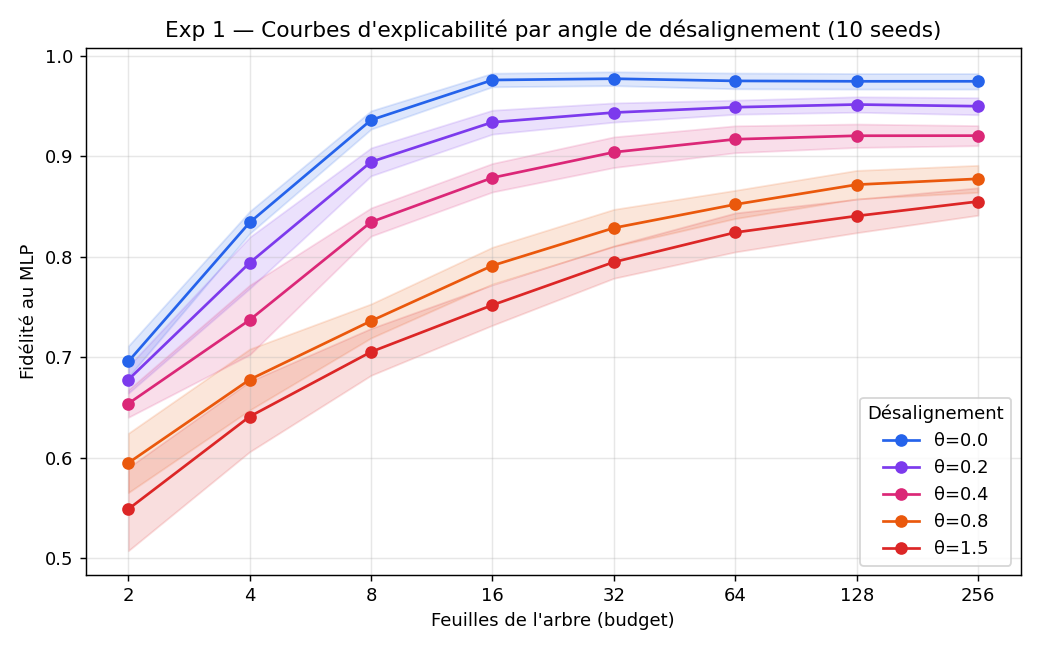
\includegraphics[width=0.62\linewidth]{exp1_courbes.png}
\caption{Experiment 1 --- explainability curves (fidelity vs.\ budget, bands $\pm$ std over 10 seeds) for receivers at increasing basis misalignment $\theta$. Not a single weight of $M$ changes across curves.}
\label{fig:exp1}
\end{figure}

\textbf{Results} (Table~\ref{tab:exp1}, Figure~\ref{fig:exp1}). The explainability AUC decreases strictly monotonically with $\theta$: $0.918$ at $\theta{=}0$ down to $0.745$ at $\theta{=}1.5$. The minimal budget for fidelity $\ge 0.95$ is 16 leaves at $\theta{=}0$, 128 at $\theta{=}0.2$, and is never reached (${>}256$) for $\theta \ge 0.4$.

\textbf{Interpretation.} Same model $M$ (not one weight changes), same information (rotations are bijections). Only the receiver's basis varies, and the explainability curves diverge monotonically with $\theta$. Explainability is therefore not a property of $M$ alone.

\subsection{Experiment 1b: what costs is mixing, not reparametrization}
\label{sec:exp1b}

Applying a coordinate-wise monotone deformation on top of the rotation ($v = \tanh(s \cdot (x - 0.5) \cdot R_{\theta=1.5})$, $s \in \{2, 6\}$, 5 seeds) leaves the AUC unchanged: $0.7432$ vs.\ $0.7433$ vs.\ $0.7433$ for the linear, $s{=}2$, and $s{=}6$ cases. For a receiver with threshold predicates, the cost of explainability is \emph{invariant under coordinate-wise monotone deformations} of its basis --- a threshold transports through any monotone function. What costs is the \emph{mixing} of dimensions, not their reparametrization: the relevant misalignment is structural, not metric. This invariance was subsequently confirmed on every test bed of this paper, synthetic and real (11 runs out of 11, often at exactly $0.0000$); a formal proof (threshold trees depend only on coordinate orders) is left to future work.

\subsection{Experiment 2: explanation as a measurable protocol}
\label{sec:exp2}

\textbf{Protocol.} Same world, same $M$; the reference graph of $M$ is a 32-leaf tree distilled in the original basis. The operator $W(x)$ answers ``why is $x$ classified $c$?'' with the decision path of $x$ (a conjunction of threshold predicates) plus its class --- minimality via the path, implicit contrast versus the other leaves. Dialogue protocol (active learning): the receiver starts from a trivial majority-class predictor; at each turn it picks a point where it disagrees with $M$, asks $W$, integrates the rule, and repeats (15 questions max, 5 seeds). The \emph{aligned} receiver stores the rule verbatim; the \emph{rotated} receiver ($\theta{=}1.5$) perceives the world only in its own basis, so each received rule --- an axis-aligned region for $M$, an oblique polytope for it --- must be approximated by a small 8-leaf tree in \emph{its} vocabulary.

\begin{table}[t]
\centering
\footnotesize
\caption{Experiment 2 --- fidelity to $M$ of the reconstructed model vs.\ number of why-questions (5 seeds). Same $M$, same answers to every query; only the receiver's basis differs.}
\label{tab:exp2}
\begin{tabular}{lcc}
\toprule
Questions & $R$ aligned & $R$ rotated ($\theta{=}1.5$) \\
\midrule
0  & $0.457{\pm}0.010$ & $0.457{\pm}0.010$ \\
3  & $0.727{\pm}0.089$ & $0.625{\pm}0.046$ \\
6  & $\mathbf{0.921{\pm}0.022}$ & $0.688{\pm}0.024$ \\
9  & $0.966{\pm}0.002$ & $0.695{\pm}0.021$ \\
12 & $0.977{\pm}0.006$ & $0.703{\pm}0.027$ \\
15 & $\mathbf{0.979{\pm}0.007}$ & $\mathbf{0.713{\pm}0.024}$ \\
\bottomrule
\end{tabular}
\end{table}

\begin{figure}[t]
\centering
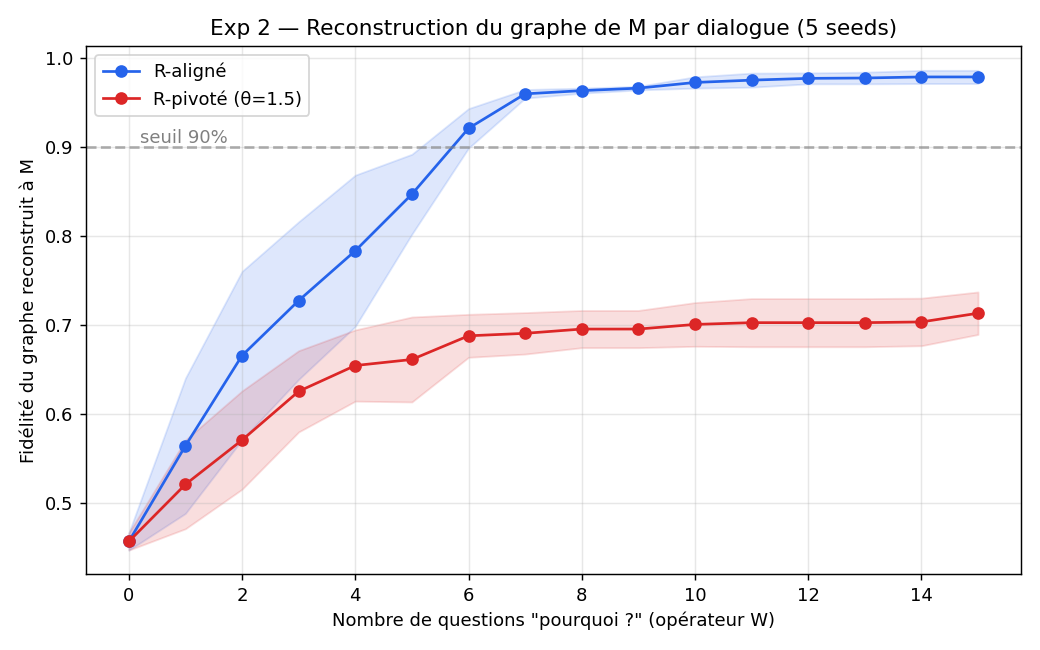
\includegraphics[width=0.58\linewidth]{exp2_dialogue.png}
\caption{Experiment 2 --- reconstruction of $M$ by successive why-questions. The aligned receiver reaches $90\%$ fidelity in 6 questions; the misaligned receiver plateaus near $71\%$ with the same answers from $M$.}
\label{fig:exp2}
\end{figure}

\textbf{Results} (Table~\ref{tab:exp2}, Figure~\ref{fig:exp2}). The aligned receiver reaches $90\%$ fidelity in 6 questions and $97.9\%$ at 15; the rotated receiver never reaches $90\%$ and plateaus at ${\sim}71\%$. Structurally, $G^\ast$ has ${\sim}7$ branches and ${\sim}6$ questions suffice: the dialogue reconstructs the structure at roughly one rule per question.

\textbf{Interpretation.} Explainability-as-protocol is measurable: the number of why-questions is small and finite when bases are aligned, and the dialogue fails to converge when they are misaligned --- \emph{with identical answers from $M$}. Two independent protocols (static distillation, interactive dialogue) confirm the same thesis.

\subsection{Experiment 4: explainability depends on the question}
\label{sec:exp4}

On the reference graph of $M$, we measure the size of the contrastive answer to ``why $a$ rather than $b$?'' --- the minimal number of diverging predicates between the instance's path and the closest path leading to $b$, weighted by leaf coverage. The answer size ranges from $2.95$ predicates (B rather than A) to $6.39$ (B rather than C), and the relation is asymmetric: A-vs-B costs $5.81$ while B-vs-A costs $2.95$. The same model is twice as ``explainable'' for some questions as for others, consistently with the pragmatic theory: explanation is not symmetric in the contrast. Full explainability should thus be defined as an expectation over the question distribution of the usage context, $\mathrm{Expl}(M, R, \bar{Q}) = \mathbb{E}_Q[\text{answer size}]$.

\section{Contact with real data: a predictive diptych}
\label{sec:real}

If misalignment is real, it should occur \emph{naturally}: some domains describe the world in compound expert concepts, others do not. The framework makes a falsifiable prediction about where an expert vocabulary should dominate a raw one --- and we tested it on two public datasets with pre-registered hypotheses and falsification criteria, reporting the negative result with the same prominence as the positive one. Both experiments use $n = 10$ seeds and per-seed paired statistics (paired $t$-test and Wilcoxon signed-rank), and both include the monotone control of Section~\ref{sec:exp1b} (log/power transforms of raw features), predicted inert.

\subsection{Experiment 5 (negative): German Credit}
\label{sec:exp5}

\textbf{Protocol.} Statlog German Credit~\citep{hofmann1994statlog}: $1{,}000$ applications, 20 attributes, binary good/bad outcome (70/30). Receiver vocabularies: \emph{raw} (features as-is); \emph{expert} = raw + compound credit concepts (installment = amount/duration, burden = installment $\times$ repayment rate, exposure = amount $\times$ number of credits); monotone control. Registered protocol v0 used an MLP ($2 \times 50$); a documented amendment v0.1 switched to gradient boosting plus $20{,}000$ extra distillation queries after the v0 MLP (accuracy $0.72$ against a $0.70$ majority class) turned out to have almost no structure to explain --- the methodological lesson, incorporated into all subsequent protocols, is to normalize the explainability curve by the fidelity of the trivial model. Falsification criterion set a priori: an expert$-$raw AUC gap below one inter-seed standard deviation means no natural misalignment on these data.

\begin{table}[t]
\centering
\footnotesize
\caption{Experiment 5 (German Credit) --- expert vs.\ raw vocabulary, $n = 10$ seeds, paired per-seed statistics. The pre-registered falsification criterion fired: a clean negative result.}
\label{tab:exp5}
\begin{tabular}{lccccc}
\toprule
Run & AUC raw & AUC expert & Paired gap & Paired $t$ & Wilcoxon \\
\midrule
v0 (MLP) & $0.733{\pm}0.025$ & $0.727{\pm}0.019$ & $-0.006{\pm}0.018$ & $p = 0.32$ & $p = 0.48$ \\
v0.1 (GBT + queries) & $0.803{\pm}0.026$ & $0.801{\pm}0.021$ & $-0.002{\pm}0.019$ & $p = 0.72$ & $p = 0.83$ \\
\bottomrule
\end{tabular}
\end{table}

\textbf{Results} (Table~\ref{tab:exp5}). No dominance of the expert vocabulary, in either run. The monotone control is inert as predicted ($-0.0008 \pm 0.0016$ in v0; $0.0000$ in v0.1) --- the invariance of Section~\ref{sec:exp1b} holds on real data.

\textbf{Interpretation.} The falsification criterion spoke: no natural misalignment on German Credit. Two readings: (a) the predictive signal of this dataset lives in categorical variables (account status, credit history) shared by both vocabularies, and the central expert concept of credit --- the debt-to-income ratio --- is not computable from the available attributes (no income); (b) more deeply, expert-vocabulary dominance requires the world's generating process to be itself written in compound quantities. That is precisely what Experiment 6 tests.

\subsection{Experiment 6 (positive): predictive maintenance}
\label{sec:exp6}

\textbf{Protocol.} AI4I 2020 Predictive Maintenance~\citep{matzka2020explainable}: $10{,}000$ points, 5 sensors (air and process temperatures, rotational speed, torque, tool wear). The benchmark's failure modes are \emph{written} in compound quantities: heat dissipation ($\Delta T$ and speed), power (torque $\times$ angular speed), overstrain (wear $\times$ torque). Hypothesis registered a priori: on physical ground --- where the generating process is written in compound quantities --- the engineer's vocabulary (sensors + $\Delta T$, power, strain) dominates the raw-sensor vocabulary; same falsification criterion as Experiment 5. Fidelity is class-balanced (failures are rare --- the lesson of Experiment 5), budgets 2 to 256 leaves, $n = 10$ seeds, paired tests, and two opaque models: an MLP ($2 \times 50$) and gradient boosting.

\begin{table}[t]
\centering
\footnotesize
\caption{Experiment 6 (AI4I 2020) --- engineer vs.\ raw vocabulary, $n = 10$ seeds, paired per-seed statistics, class-balanced fidelity. The gap depends on the internal basis of $M$ itself.}
\label{tab:exp6}
\begin{tabular}{lccccc}
\toprule
$M$ & AUC raw & AUC engineer & Paired gap & Paired $t$ & Wilcoxon \\
\midrule
MLP & $0.702{\pm}0.050$ & $0.748{\pm}0.048$ & $\mathbf{+0.046{\pm}0.026}$ & $t = 5.37$, $p = 4.5{\times}10^{-4}$ & $p = 0.002$ \\
GBT & $0.760{\pm}0.022$ & $0.755{\pm}0.017$ & $-0.005{\pm}0.027$ & $p = 0.56$ & $p = 0.56$ \\
\bottomrule
\end{tabular}
\end{table}

\begin{figure}[t]
\centering
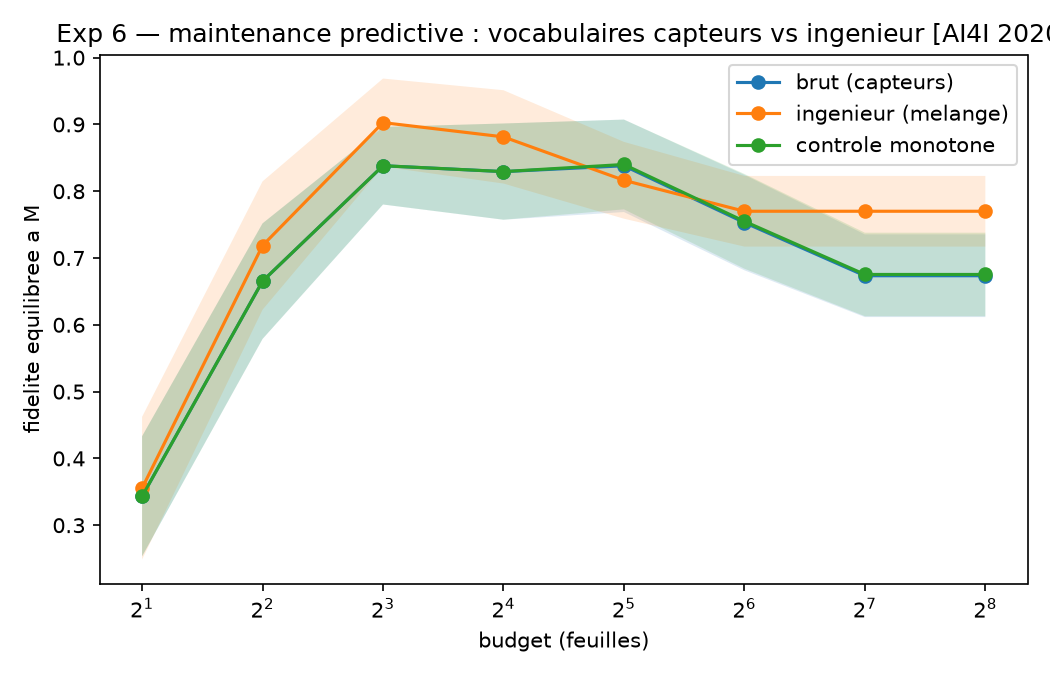
\includegraphics[width=0.62\linewidth]{exp6_ai4i.png}
\caption{Experiment 6 --- explainability curves on AI4I 2020 for raw vs.\ engineer vocabularies (class-balanced fidelity, 10 seeds). The engineer's vocabulary dominates for the MLP; the gap vanishes for the axis-aligned GBT.}
\label{fig:exp6}
\end{figure}

\textbf{Results} (Table~\ref{tab:exp6}, Figure~\ref{fig:exp6}). For the MLP, the engineer's vocabulary dominates ($+0.046 \pm 0.026$, paired $t = 5.37$, $p = 4.5{\times}10^{-4}$, Wilcoxon $p = 0.002$). For gradient boosting, the gap vanishes ($-0.005 \pm 0.027$, $p = 0.56$). Monotone controls are inert in both cases. Balanced accuracy of $M$ is $0.62$ (MLP) and $0.71$ (GBT); the residual failure modes of AI4I are known to be nearly unlearnable.

\textbf{Interpretation.} To our knowledge, this is the first controlled demonstration of \emph{natural} basis misalignment on real data. Together with Experiment 5 it forms a diptych: no dominance where the world is not written in compound concepts (credit), clear dominance where it is (physics) --- natural misalignment exists, and the framework predicts where. The GBT result is the structural surprise: a tree ensemble is built from axis-aligned splits on raw features --- \emph{its internal basis is the raw vocabulary by construction} --- and the gap disappears; the MLP mixes dimensions the way the physics does, and the gap appears. Same data, same receivers, different $M$, different explainability relation: the relational thesis observed \emph{on the model side}, everything else held fixed. Caveats: one dataset per verdict; expert vocabularies chosen by the authors, not learned; rare classes limit the learnable structure of $M$.

\section{The interactive regime: the channel that explains is the channel that learns}
\label{sec:interactive}

The why-operator has an inverse: where $W$ extracts a rule from $M$'s explainable graph, $W^{-1}$ inserts or edits one, supplied by the receiver in the shared vocabulary. Because an edit touches exactly the rules it names, regions outside the edit are intact \emph{by construction} --- catastrophic forgetting~\citep{mccloskey1989catastrophic,french1999catastrophic} is not mitigated, it is removed. This section tests the resulting learning regime, first on a single correction, then under continuous drift.

\subsection{Experiment 3: one sentence vs.\ thousands of examples}
\label{sec:exp3}

\textbf{Protocol (concept drift).} The world changes: the rule ``shape $> 0.7 \to$ B'' of $G^\ast$ becomes ``shape $> 0.7 \to$ A''. $M$, trained on the old world, drops to $0.741$ accuracy. Route A (our framework): the explainable graph of $M$ (rule list extracted from the 32-leaf reference tree) is corrected by \emph{one} sentence of dialogue --- ``when shape $> 0.7$, it is A now'' --- implemented as $W^{-1}$ editing the class of the concerned rules; cost: one interaction, zero gradients. Route B (standard paradigm): the MLP is fine-tuned (warm start, 50 epochs) on $n \in \{10, \dots, 3000\}$ freshly labeled examples. Accuracy on the new world, 5 seeds.

\begin{table}[t]
\centering
\footnotesize
\caption{Experiment 3 --- adaptation to a rule flip: one graph edit through dialogue vs.\ fine-tuning on labeled examples (5 seeds).}
\label{tab:exp3}
\begin{tabular}{lcc}
\toprule
Method & Cost & Accuracy (new world) \\
\midrule
$M$ without adaptation & --- & $0.741{\pm}0.012$ \\
\textbf{Graph edit (dialogue)} & \textbf{1 sentence} & $\mathbf{0.990{\pm}0.004}$ \\
Fine-tuning & 10 examples & $0.758{\pm}0.046$ \\
Fine-tuning & 100 examples & $0.893{\pm}0.012$ \\
Fine-tuning & 1000 examples & $0.947{\pm}0.004$ \\
Fine-tuning & 3000 examples & $0.968{\pm}0.004$ \\
\bottomrule
\end{tabular}
\end{table}

\textbf{Results} (Table~\ref{tab:exp3}). One sentence of dialogue outperforms $3{,}000$ examples of fine-tuning ($0.990$ vs.\ $0.968$). The edit is instantaneous, local, and traceable.

\textbf{Methodological fair play.} The comparison is deliberately \emph{not} information-equal: one semantic sentence compresses what thousands of examples express --- that is the thesis, not a confound. The explanation channel ($W$) and the learning channel ($W^{-1}$) are the same channel used in both directions. Note also that Route A requires the correction to be expressible in the shared vocabulary: under a misaligned basis (Experiments 1--2) this channel degrades, which ties the experiments into a single narrative --- and Experiment 7 quantifies exactly that tax.

\subsection{Experiment 7: a graph maintained by dialogue under continuous drift}
\label{sec:exp7}

\textbf{Protocol (pre-registered; kill conditions published before the run --- the git record is the evidence).} The reference world $G^\ast$ undergoes 15 successive drifts: at each step the class of one branch flips (deterministic cyclic schedule). Competitors: (a) the explainable graph (32 leaves distilled from the initial $M$) maintained by dialogue --- \emph{one} sentence per drift (``in the region $\langle$branch condition$\rangle$, the class is now $c$''), interpreted against the receiver's own unlabeled experience (any rule whose firing region lies mostly inside the sentence's region is re-classed); zero labeled examples; (b) the frozen MLP; (c) the MLP fine-tuned on 100 fresh labeled examples per drift (50 epochs); (d) the MLP retrained from scratch on $5{,}000$ examples per drift. 5 seeds. Stress variants: noisy sentences (thresholds perturbed by $\pm 0.05$ and $\pm 0.10$ --- human imprecision); receiver in a misaligned basis ($\theta = 1.5$). Four kill conditions were set a priori: K1, the graph falls below fine-tuning over the last 5 drifts; K2, accuracy of a never-edited region degrades after 15 edits; K3, the advantage over the frozen model vanishes under $\pm 0.10$ noise; K4, the misaligned graph falls below the frozen model.

\begin{table}[t]
\centering
\footnotesize
\caption{Experiment 7 --- mean accuracy over 15 drifts (5 seeds). The dialogue-maintained graph uses 15 sentences and zero labels; all four pre-registered kill conditions survived.}
\label{tab:exp7}
\begin{tabular}{lcc}
\toprule
Method & Total supervision (15 drifts) & Mean accuracy (drifts 1--15) \\
\midrule
Frozen MLP & --- & $0.624{\pm}0.002$ \\
Fine-tuned MLP & $1{,}500$ labels & $0.854{\pm}0.018$ (forgetting sawtooth, min $0.740$) \\
Retrained-from-scratch MLP & $75{,}000$ labels & $0.981{\pm}0.002$ \\
\textbf{Graph + dialogue} & \textbf{15 sentences, 0 labels} & $\mathbf{0.990{\pm}0.003}$ \\
Graph, noisy sentences $\pm 0.05$ & 15 sentences & $0.984{\pm}0.008$ \\
Graph, noisy sentences $\pm 0.10$ & 15 sentences & $0.971{\pm}0.018$ \\
Graph, misaligned basis $\theta{=}1.5$ & 15 sentences & $0.801{\pm}0.028$ \\
\bottomrule
\end{tabular}
\end{table}

\begin{figure}[t]
\centering
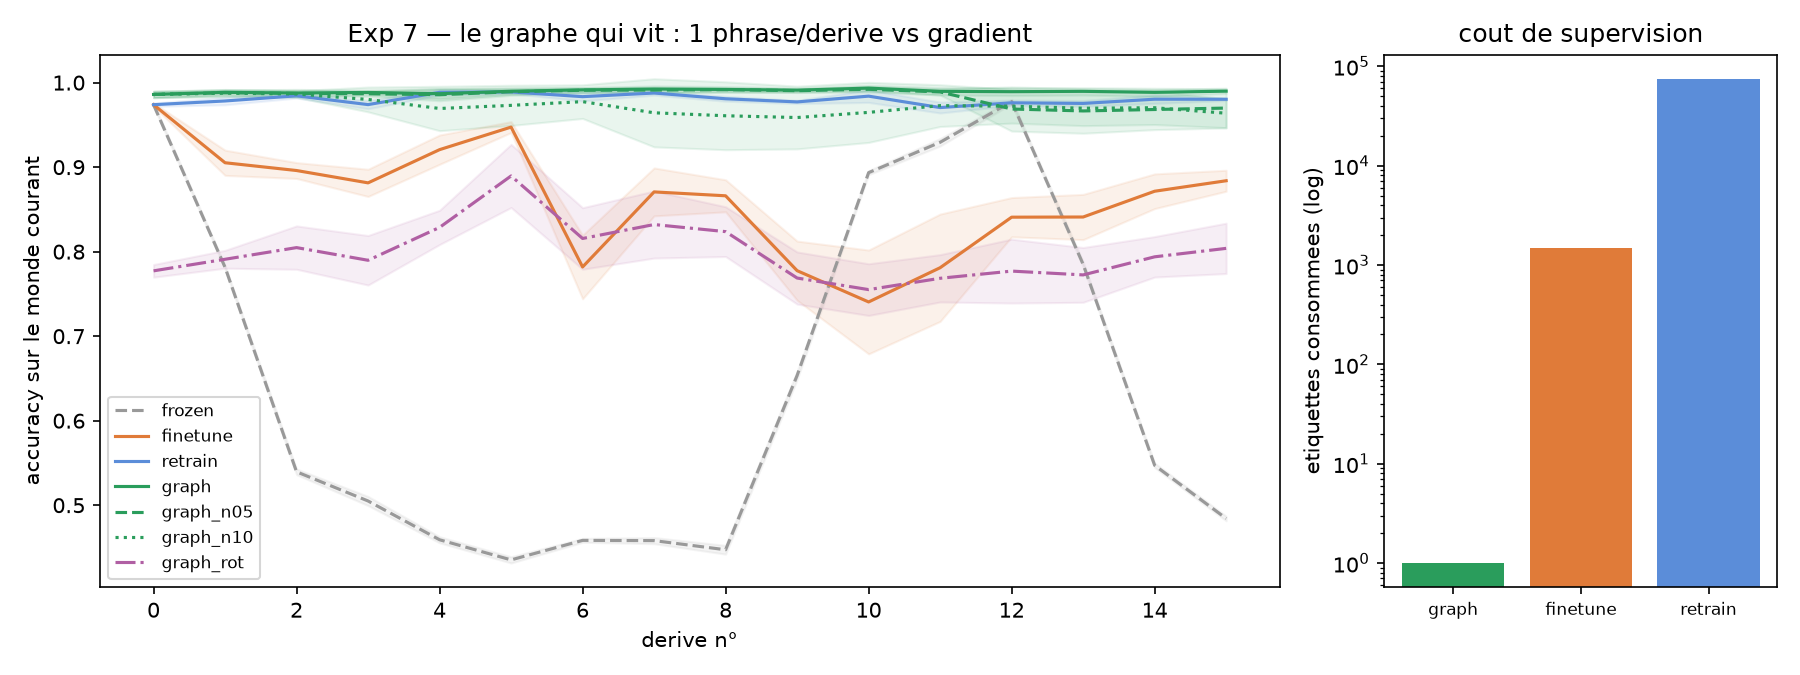
\includegraphics[width=0.66\linewidth]{exp7_living_graph.png}
\caption{Experiment 7 --- accuracy along 15 successive drifts for the four competitors and the stress variants. The dialogue-maintained graph (15 sentences, zero labels) dominates throughout; the never-edited region shows zero cumulative degradation.}
\label{fig:exp7}
\end{figure}

\textbf{Results} (Table~\ref{tab:exp7}, Figure~\ref{fig:exp7}). Fifteen sentences with zero labels outperform $75{,}000$ labels of from-scratch retraining ($0.990 \pm 0.003$ vs.\ $0.981 \pm 0.002$). All four kill conditions survived. Integrity of the never-edited region after 15 edits: $0.992 \to 0.994$ --- zero cumulative degradation (K2: locality holds over 15 edits). Human imprecision of $\pm 0.10$ costs only ${\sim}2$ points ($0.971$). The misaligned receiver pays a measured \emph{expressibility tax} of ${\sim}0.19$ ($0.801$), quantitatively linking Experiments 1--2 to Experiment 3. An unplanned control: the cyclic schedule returns the world to its initial state at drift 12, where the frozen model climbs back exactly to its original level --- the drift mechanics are sound.

\textbf{The conjecture, stated as such.} We conjecture that learning by graph editing in dialogue is a \emph{candidate paradigm for post-gradient learning}: data-efficient because the channel is semantic, and continual by construction because edits are local. It attacks head-on the two best-documented weaknesses of deep learning --- data inefficiency (one sentence compresses thousands of examples, Experiment 3) and catastrophic forgetting (locality removes the problem rather than mitigating it, Experiment 7 / K2). This is a conjecture supported by controlled synthetic evidence, not an established claim.

\section{Limitations}
\label{sec:limits}

\begin{itemize}
  \item Synthetic experiments are low-dimensional with $G^\ast$ known by construction. This is a choice --- total control of misalignment, impossible with human subjects --- but generalization to high dimension remains to be demonstrated.
  \item Receivers are artificial. Human validation (experts vs.\ novices as different bases) is the next step, not the present contribution; no claim in this paper concerns human receivers.
  \item Misalignment is modeled by linear rotations (plus monotone deformations); real conceptual misalignments are nonlinear and structured.
  \item The ``graph of $M$'' is a high-fidelity distilled proxy, not the exact network.
  \item Experiment 3's dialogue/fine-tuning comparison is not information-equal (assumed --- it is the thesis), and identifying the rule to edit is assisted by knowledge of $G^\ast$; in real conditions, localizing the faulty rule is a problem in itself.
  \item The performance--interpretability trade-off~\citep{rudin2019stop}: our synthetic worlds are compressible by construction. The thesis ``an interactive graph beats a frozen network under continual learning'' is now tested in a synthetic regime (Experiment 7), not yet on real streams.
  \item Experiments 5--6: one dataset per verdict of the diptych; expert vocabularies are chosen by the authors, not learned; on AI4I, near-random residual failure modes limit the learnable structure of $M$.
  \item Experiment 7: sentences come from an oracle that localizes the concerned region (noisy variants tested; autonomous localization unresolved); the receiver has the world's inductive bias --- the $\theta = 1.5$ variant prices the opposite case.
\end{itemize}

\section{Perspectives and conclusion}
\label{sec:conclusion}

One line each, in order of priority: human validation of the framework (simulatability measured on subjects, bases operationalized by expertise); autonomous localization of the rule to edit when the correction does not name it; more datasets per verdict of the real-data diptych, with \emph{learned} rather than chosen expert vocabularies; a formal proof of the monotone-invariance proposition and a characterization of the cost by mixing structure (angles between subspaces); contextual compression of large models --- ``the best graph of size $K$ for context $C$'' --- as a primitive; weighting explainability by realistic question distributions $Q$; construction of a common basis through a bilateral feedback loop, superposition of crisp graphs as a model of vague language, and a calibration operator; and the connection to interactive proofs and debate~\citep{irving2018ai}, with the receiver as a bounded verifier.

Explainability research keeps asking what a model must look like to be understandable. We propose to ask, instead, \emph{for whom} it is understandable — and to make the receiver a first-class citizen of the definition. Once the receiver is in the equation, explanation stops being a report and becomes a channel: measurable in questions (Experiments 1--2, 4), predictive on real data in both directions (Experiments 5--6, including a clean pre-registered negative result), sensitive to the model's own internal basis (Experiment 6), and reversible into a learning mechanism whose locality abolishes forgetting by construction (Experiments 3, 7). The evidence presented here is deliberately preliminary — controlled worlds, artificial receivers, honest kill conditions — but the direction is stated without hedging: there is no explainability without a receiver.

\subsection*{Reproducibility}
\label{sec:repro}

All experiments (10 or 5 seeds, fixed), the \texttt{rex} library (rule-list model, $W$, $W^{-1}$, metrics, with unit tests including the edit-locality invariant), figures, and dataset download scripts are available at \url{https://github.com/RedaAZIZI/impact_social}. Experiment 7's hypotheses and kill conditions were pre-registered in the repository before the run; Experiment 5's protocol amendment (v0 $\to$ v0.1) is documented in the same place. No dataset is redistributed; both real datasets are public UCI benchmarks~\citep{hofmann1994statlog,matzka2020explainable}.

\subsection*{Acknowledgments}

The author thanks Anthropic's Claude for assistance with implementation, formalization, and manuscript preparation. The vision, the framework, and the scientific decisions are the author's.

\bibliographystyle{unsrtnat}
\setlength{\bibsep}{2.5pt}
{\footnotesize
\bibliography{references}}

\end{document}
